\documentclass[12pt, a4paper]{article}
\usepackage[utf8]{inputenc}
\usepackage[russian]{babel}
\usepackage[pdftex]{graphicx, color}
\usepackage{amsmath}
\usepackage{amsfonts}
\usepackage{amssymb}
\usepackage{amsthm}
\usepackage[left=2cm,right=1.5cm,top=1.5cm,bottom=2cm]{geometry}
\usepackage{indentfirst}
\usepackage{hyperref}

\usepackage{pbox}

\usepackage{setspace}
\onehalfspacing
\graphicspath{{pic/}}

\begin{document}

	\thispagestyle{empty}

	\begin{singlespace}
	\begin{titlepage}
		\begin{center}
			
\includegraphics[height = 3cm]{msu.png}

			{\scshape Московский государственный университет имени М.~В.~Ломоносова}\\
			Факультет вычислительной математики и кибернетики\\
			\centerline{\hfill\hrulefill\hrulefill\hrulefill\hrulefill\hfill}

			\vfill

			{\LARGE Отчет к первому практическому заданию по БММО: \\ Байесовские рассуждения}

			\vspace{1cm}

		\end{center}

		\vfill
		\begin{flushright}
			\textit{Студент 4 курса ВМК (417 группа):}\\
				Оспанов А.М.

			\vspace{5mm}

		\end{flushright}

		\vfill

		\begin{center}
		Москва, 2015
		\end{center}
	\end{titlepage}
	\end{singlespace}

	\tableofcontents


	\newpage
	\section{Введение}
		Данный отчет написан к первому практическому заданию по БММО. Тема задания: Байесовские рассуждения. Отчет написан студентом 417 группы -- Оспановым Аятом.

		В данной работе были реализованы 3 и 4 вероятностные модели посещаемости курса. Были сделаны все исследования, требуемые в задании. Ipython Notebook-и поделены на 2, т.е. каждая модель в своем Notebook-е.

	\newpage
	\section{Основная часть}
		\subsection{Математические ожидания и дисперсии}
			Математические ожидания и дисперсии для моделей считались аналитический. Применялись следующие свойства условного матожидания и условной дисперсии:
			$$\mathbb{E} X = \mathbb{E}\mathbb{E} [X | Y]$$
			$$\mathbb{D} X = \mathbb{E}\mathbb{D} [X | Y] + \mathbb{D}\mathbb{E} [X | Y]$$
			
			В результате получились следующие формулы для вычисления матожиданий и дисперсий:
		
			\begin{itemize}
			    \item Для модели 3:
			    $$\mathbb{E} a = \frac{a_{max} + a_{min}}{2}$$
			    $$\mathbb{E} b = \frac{b_{max} + b_{min}}{2}$$
			    $$\mathbb{E} c_n = p_1 \mathbb{E} a + p_2 \mathbb{E} b$$
			    $$\mathbb{E} d_n = (1 + p_3)\mathbb{E} c_n$$
			    
			    $$\mathbb{D} a = \frac{(a_{max} - a_{min} + 1)^2 + 1}{12}$$
			    $$\mathbb{D} b = \frac{(b_{max} - b_{min} + 1)^2 + 1}{12}$$
			    $$\mathbb{D} c_n = p_1 (1 - p_1) \mathbb{E} a + p_2 (1 - p_2) \mathbb{E} b + p_1^2 \mathbb{D} a + p_2^2 \mathbb{D} b$$
			    $$\mathbb{D} d_n = p_3 (1 - p_3)\mathbb{E} c_n + (1 + p_3)^2 \mathbb{D} c_n$$
			    \item Для модели 4 (различается только $\mathbb{D} c_n$):
			    $$\mathbb{D} c_n = p_1 \mathbb{E} a + p_2 \mathbb{E} b + p_1^2 \mathbb{D} a + p_2^2 \mathbb{D} b$$
			\end{itemize}
			\begin{center}
			\begin{tabular}{| l | c | c |}
				\hline
  				& Модель 3 & Модель 4 \\
  				\hline
  				$\mathbb{E} a$ & 82.5 & 82.5 \\
  				\hline
  				$\mathbb{E} b$ & 550.0 & 550.0 \\
  				\hline
  				$\mathbb{E} c_n$ & 13.75 & 13.75 \\
  				\hline
  				$\mathbb{E} d_n$ & 17.875 & 17.875 \\
  				\hline
  				$\mathbb{D} a$ & 21.25 & 21.25 \\
  				\hline
  				$\mathbb{D} b$ & 850.0 & 850.0 \\
  				\hline
  				$\mathbb{D} c_n$ & 13.1675 & 14.0475 \\
  				\hline
  				$\mathbb{D} d_n$ & 25.1405 & 26.6277 \\
  				\hline
			\end{tabular}
			\end{center}

		\newpage
		\subsection{Наблюдение $p(b|d_1, ..., d_N), p(d|a, d_1, ..., d_N)$}
			\begin{center}
			
			$d_1, ..., d_N$ сгенерирована из модели при параметрах $a = \mathbb{E}a, b = \mathbb{E}b$
			
			\textbf{Математические ожидания}
			\begin{tabular}{ c  c }
  				Модель 3 & Модель 4 \\
  				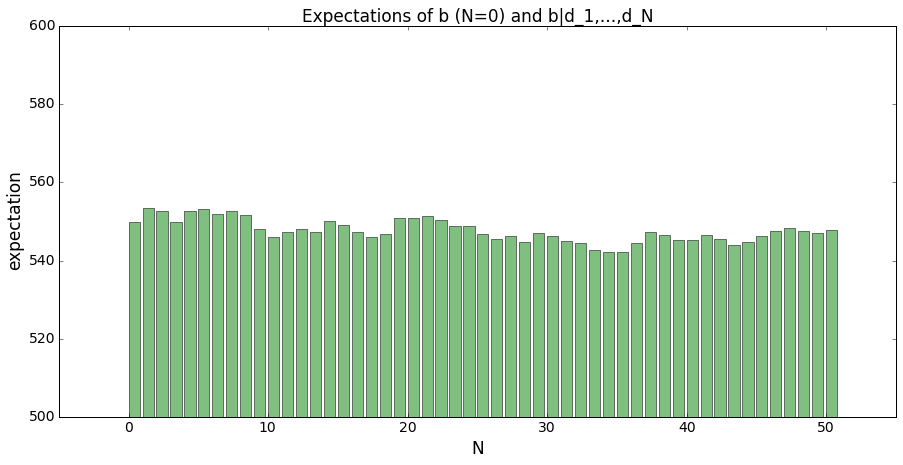
\includegraphics[width=8.5cm]{expec_m3_d_gen.png} &
  				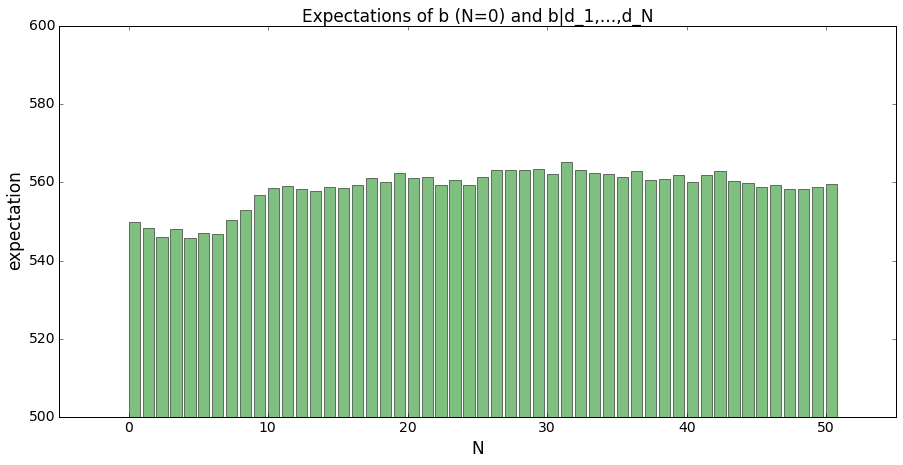
\includegraphics[width=8.5cm]{expec_m4_d_gen.png} \\
  			\end{tabular}
  			
  			При известном a (для исследования считалось $a = \mathbb{E}a$)
  			\begin{tabular}{ c  c }
  				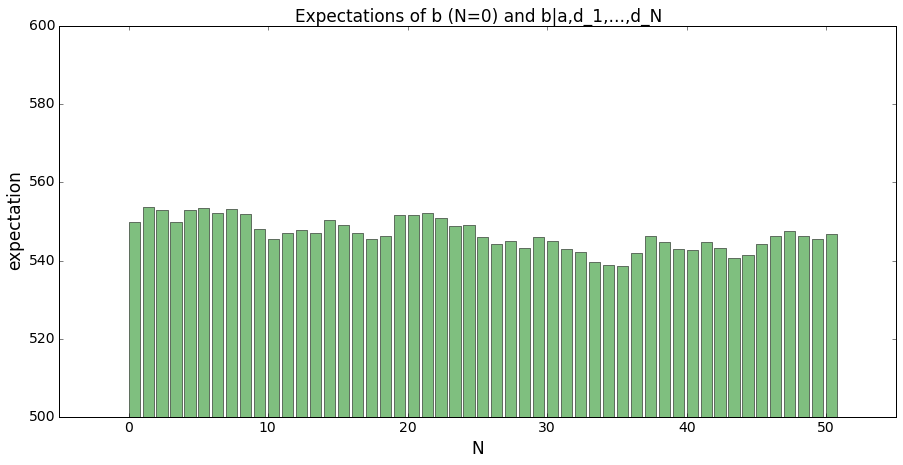
\includegraphics[width=8.5cm]{expec_m3_ad_gen.png} &
  				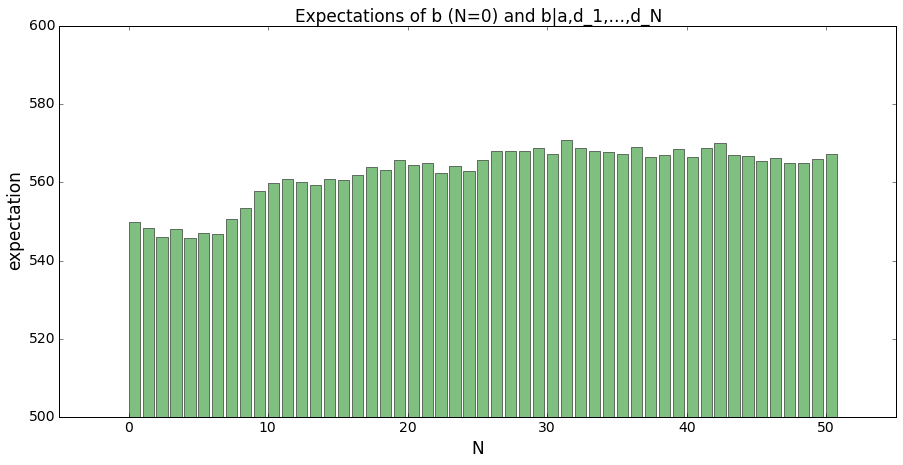
\includegraphics[width=8.5cm]{expec_m4_ad_gen.png} \\
			\end{tabular}
			
			\textbf{Дисперсии}
			\begin{tabular}{ c  c }
  				Модель 3 & Модель 4 \\
  				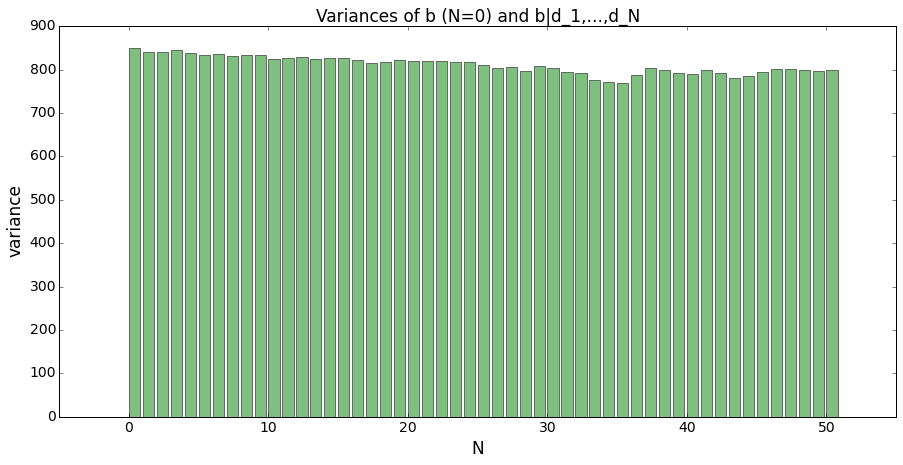
\includegraphics[width=8.5cm]{var_m3_d_gen.png} &
  				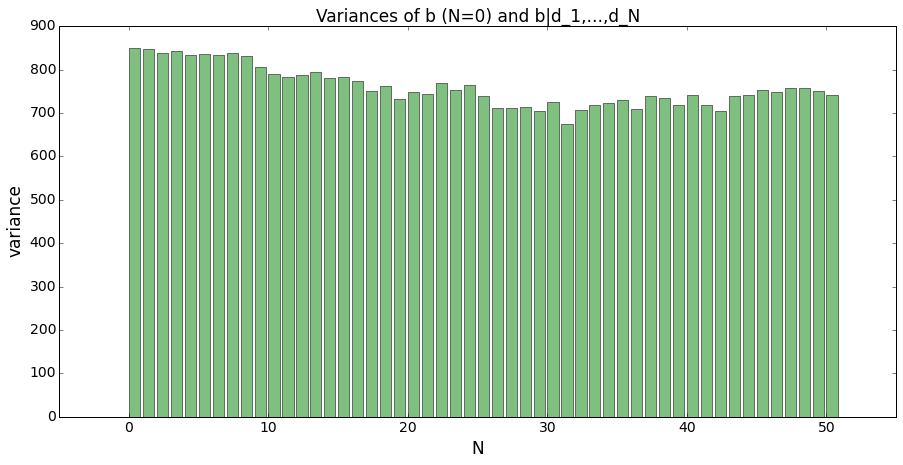
\includegraphics[width=8.5cm]{var_m4_d_gen.png} \\
  			\end{tabular}
  			При известном a (для исследования считалось $a = \mathbb{E}a$)
  			\begin{tabular}{ c  c }
  				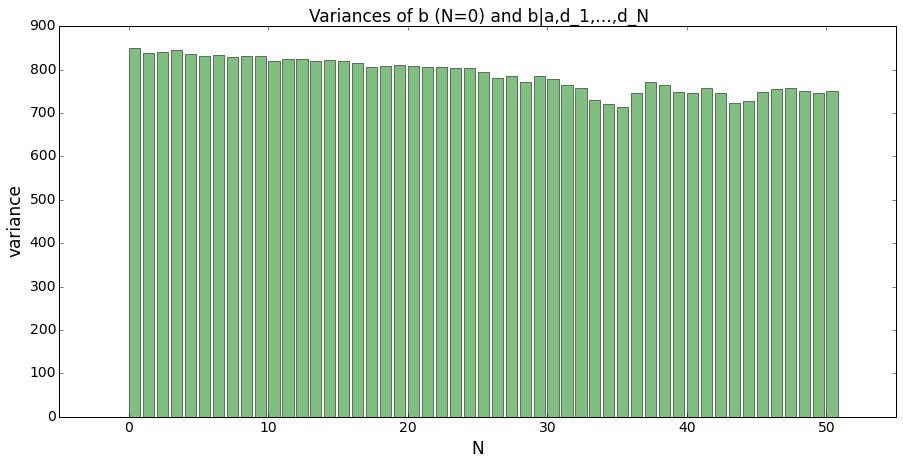
\includegraphics[width=8.5cm]{var_m3_ad_gen.png} &
  				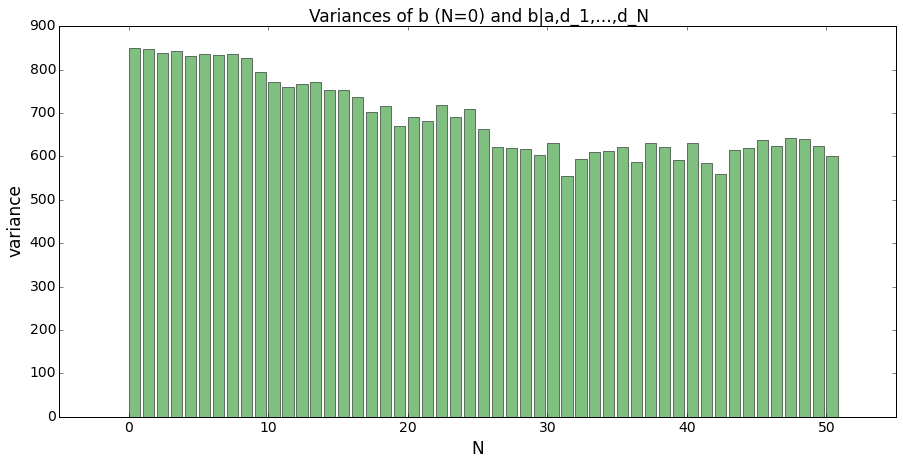
\includegraphics[width=8.5cm]{var_m4_ad_gen.png} \\
			\end{tabular}
			
			\end{center}
			
			Из математических ожиданий $b|d_1, ..., d_N$ для модели 3 можно увидеть, что среднее количество студентов других факультетов уменьшается с добавлением $d_i$. Но при этом, в среднем, матожидение находится около 550, т.е. матожидания априорного распределения. А в модели 4 матожидание завышено (в этом мы убедимся и в дальнейших исследованиях). Если дополнительно известно значение а (в нашем случае берется матожидение априорного распределения $a$), то матожидание практический не меняется. Это можно объяснить тем, что $a$ и $b$ независимы.
			
			Дисперсии же убывают с добавлением $d_i$, т.е. чем больше нам известно об отметившихся студентах, тем с большей точностью мы можем предсказать $b$.
			
			\newpage
			\begin{center}
			$d_1 = ... = d_N = \mathbb{E} d_N$
			
			\textbf{Математические ожидания}
			\begin{tabular}{ c  c }
  				Модель 3 & Модель 4 \\
  				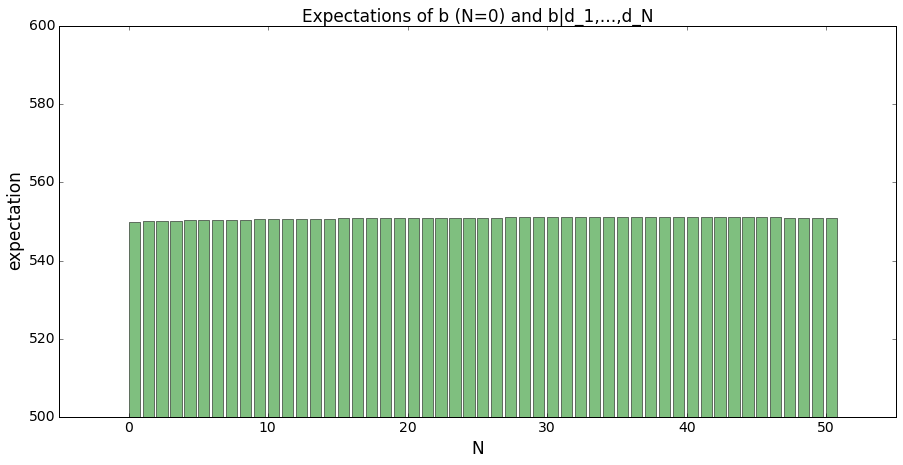
\includegraphics[width=8.5cm]{expec_m3_d_ex.png} &
  				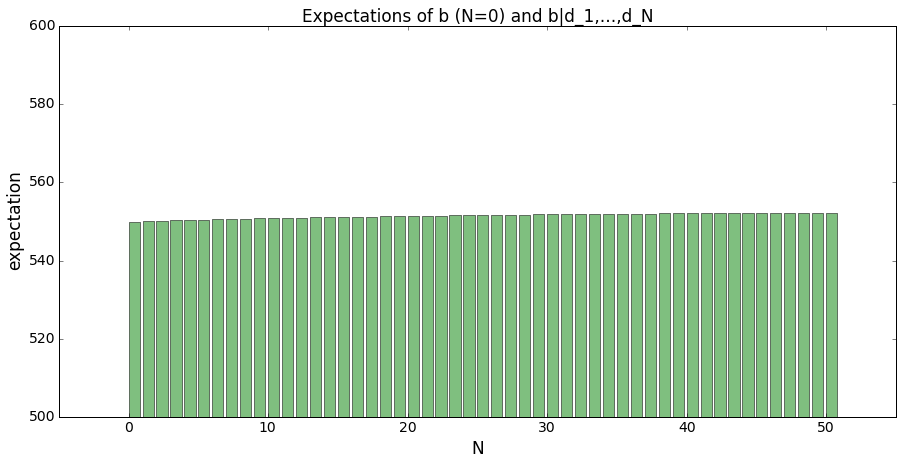
\includegraphics[width=8.5cm]{expec_m4_d_ex.png} \\
  			\end{tabular}
  			При известном a (для исследования считалось $a = \mathbb{E}a$)
  			\begin{tabular}{ c  c }
  				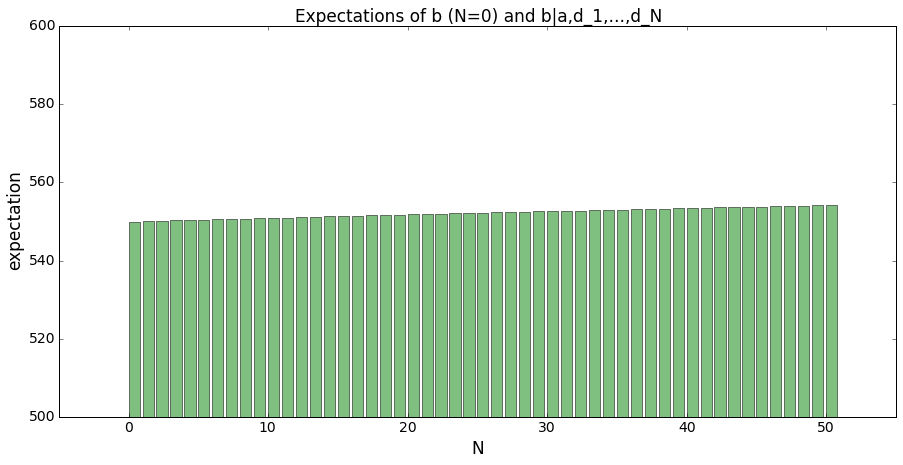
\includegraphics[width=8.5cm]{expec_m3_ad_ex.png} &
  				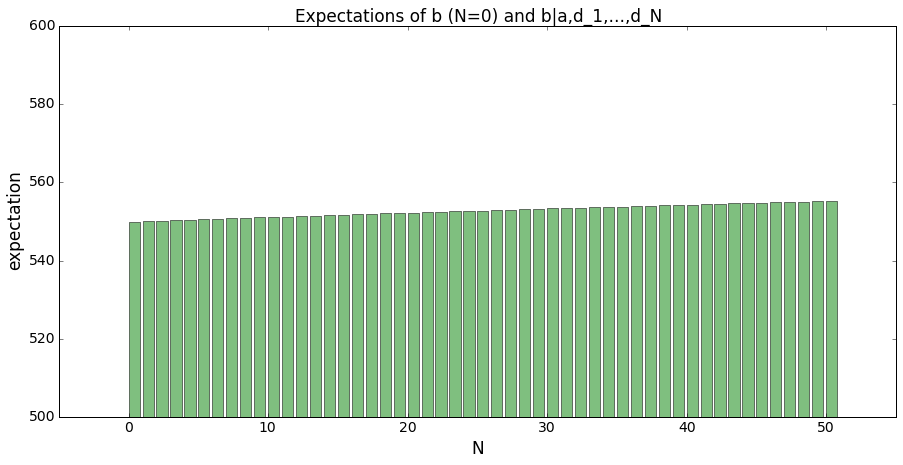
\includegraphics[width=8.5cm]{expec_m4_ad_ex.png} \\
			\end{tabular}
			
			\textbf{Дисперсии}
			\begin{tabular}{ c  c }
  				Модель 3 & Модель 4 \\
  				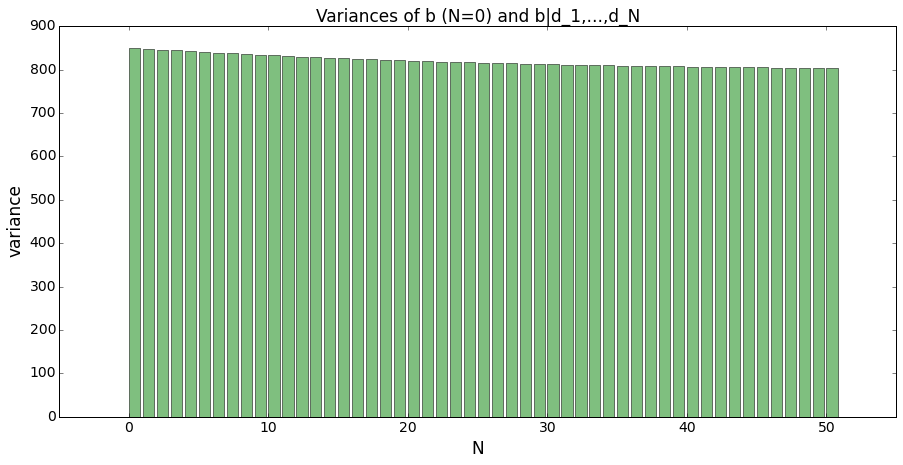
\includegraphics[width=8.5cm]{var_m3_d_ex.png} &
  				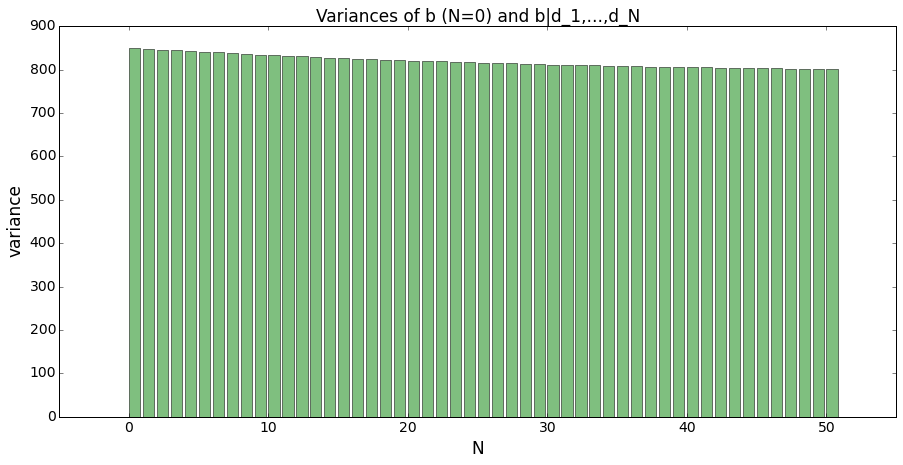
\includegraphics[width=8.5cm]{var_m4_d_ex.png} \\
  			\end{tabular}
  			При известном a (для исследования считалось $a = \mathbb{E}a$)
  			\begin{tabular}{ c  c }
  				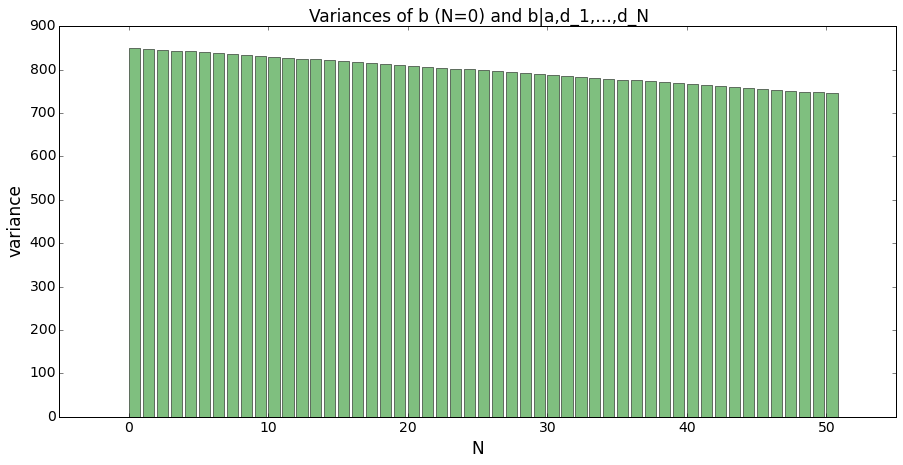
\includegraphics[width=8.5cm]{var_m3_ad_ex.png} &
  				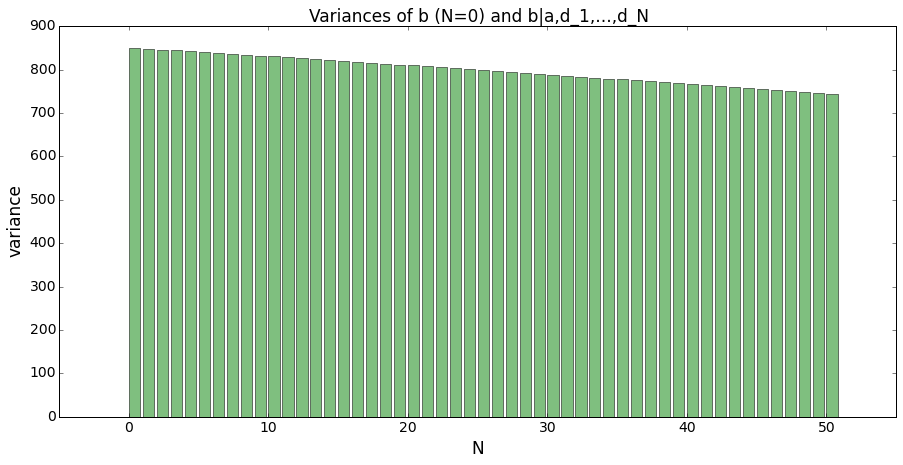
\includegraphics[width=8.5cm]{var_m4_ad_ex.png} \\
			\end{tabular}
			\end{center}
			
			В случае равных значений $d_i$ модели практически одинаковые, а матожидания и дисперсии монотонны.
			
			\newpage
			\begin{center}
			$d_1, ..., d_N$ сгенерирована из модели при параметрах $a = \mathbb{E}a, b = \mathbb{E}b$
			
			\begin{tabular}{ c  c }
  				Модель 3 & Модель 4 \\
  				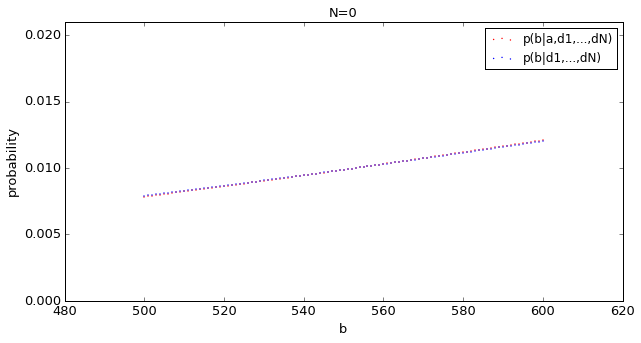
\includegraphics[width=8cm, height=4cm]{graphs/m3_gen_n0.png} &
  				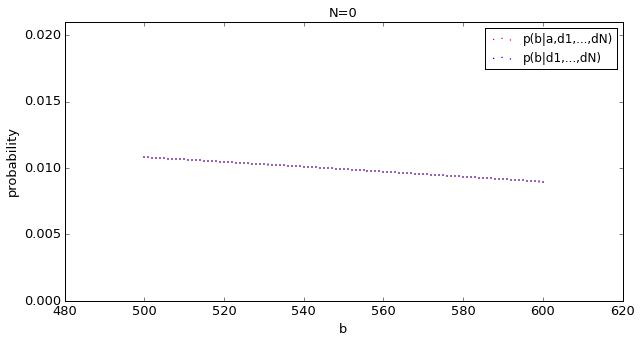
\includegraphics[width=8cm, height=4cm]{graphs/m4_gen_n0.png} \\
  				
  				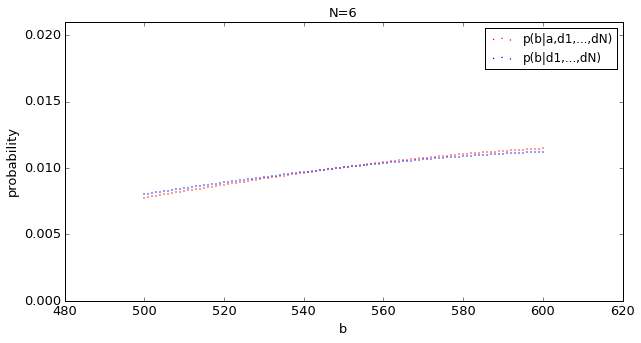
\includegraphics[width=8cm, height=4cm]{graphs/m3_gen_n6.png} &
  				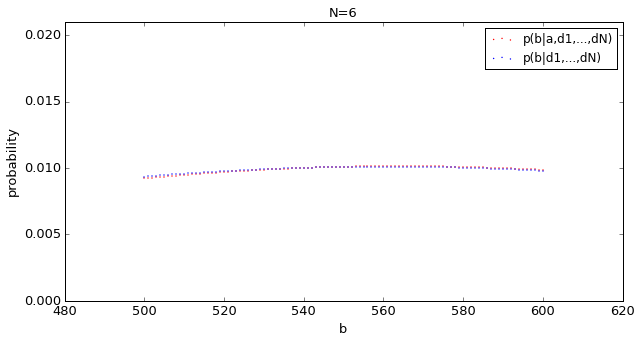
\includegraphics[width=8cm, height=4cm]{graphs/m4_gen_n6.png} \\
  				
  				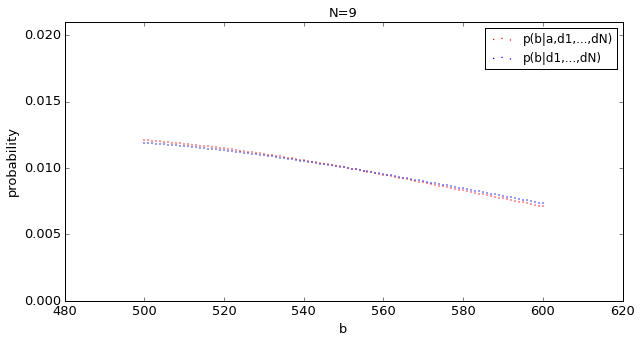
\includegraphics[width=8cm, height=4cm]{graphs/m3_gen_n9.png} &
  				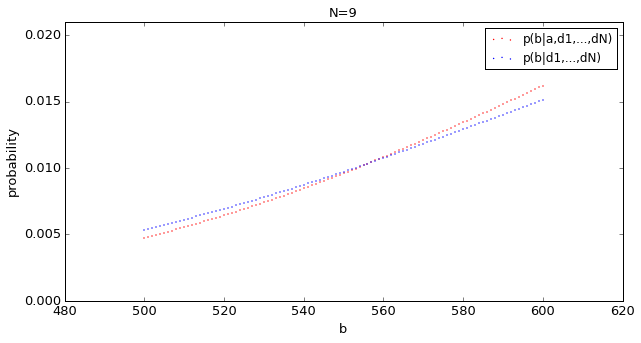
\includegraphics[width=8cm, height=4cm]{graphs/m4_gen_n9.png} \\
  				
  				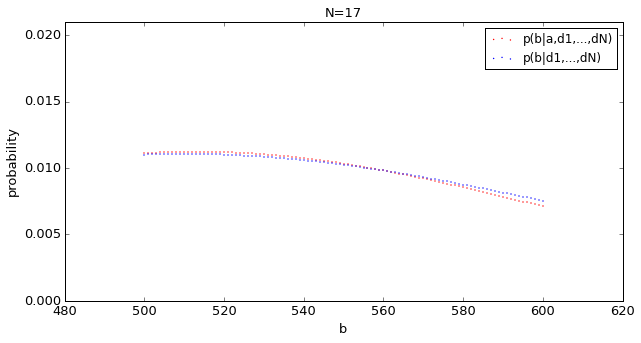
\includegraphics[width=8cm, height=4cm]{graphs/m3_gen_n16.png} &
  				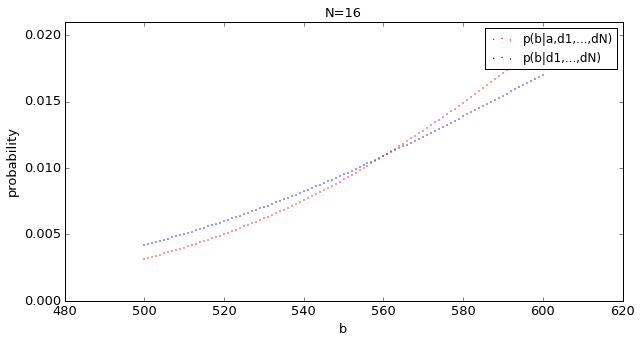
\includegraphics[width=8cm, height=4cm]{graphs/m4_gen_n16.png} \\
  				
  				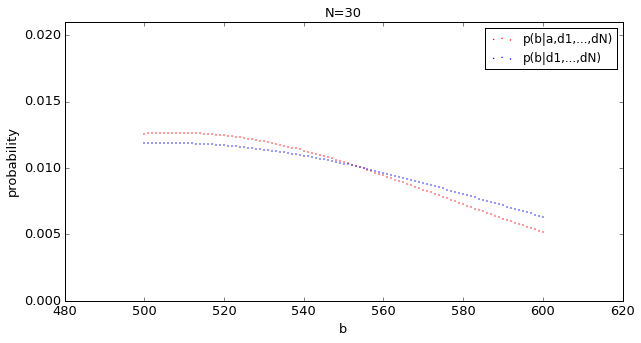
\includegraphics[width=8cm, height=4cm]{graphs/m3_gen_n30.png} &
  				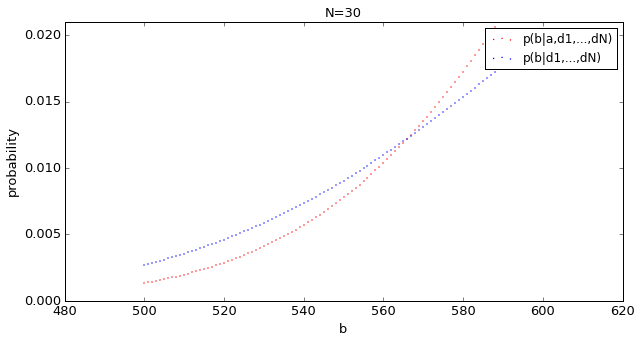
\includegraphics[width=8cm, height=4cm]{graphs/m4_gen_n30.png} \\
  				
  				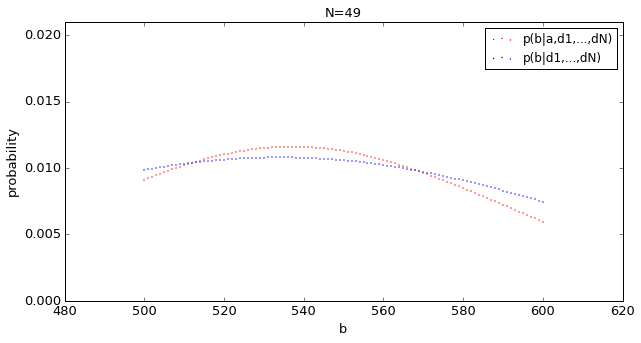
\includegraphics[width=8cm, height=4cm]{graphs/m3_gen_n49.png} &
  				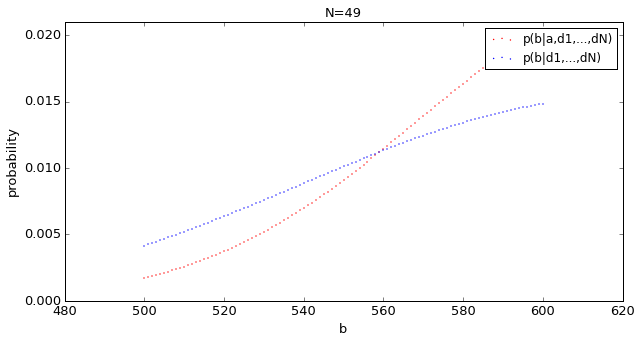
\includegraphics[width=8cm, height=4cm]{graphs/m4_gen_n49.png} \\
			\end{tabular}
			\end{center}
			
			Теперь рассмотрим плотности распределний $b|a,d_1,...,d_N$ и $b|d_1,...,d_N$. Здесь мы можем видеть, что в модели 3, при добавлении $d_i$, вероятность того, что студентов других факультетов будет больше матожидания $b$ уменьшается. Но в модели 4, эта вероятность растет. Т.е. погрешность прибилжения суммы биномиальных распределений Пуассоновским распределением - большая.
			
			Также, если дополительно известно значение $a$, то график практический не меняется. Это также объясняется независимостью $a$ и $b$ .
			
			\newpage
			\begin{center}
			$d_1 = ... = d_N = \mathbb{E} d_N, a = \mathbb{E}a$
			
			\begin{tabular}{ c  c }
  				Модель 3 & Модель 4 \\
  				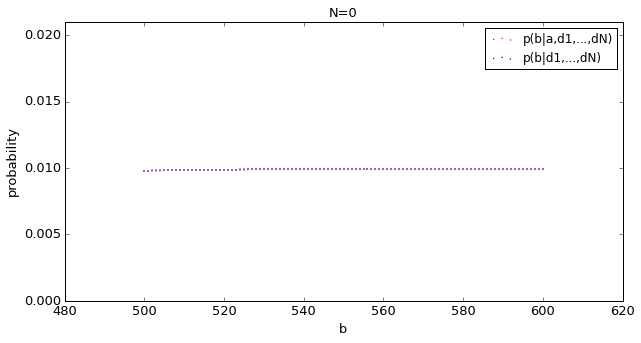
\includegraphics[width=8cm, height=4cm]{graphs/m3_ex_n0.png} &
  				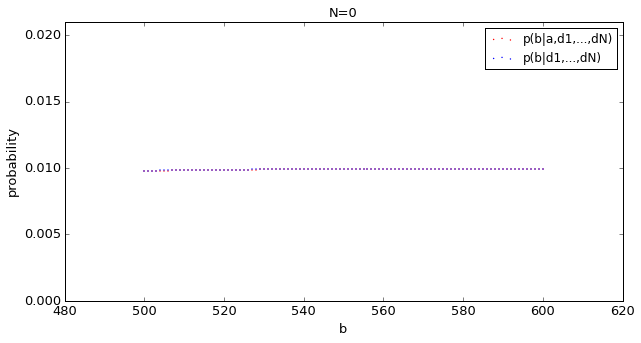
\includegraphics[width=8cm, height=4cm]{graphs/m4_ex_n0.png} \\
  				
  				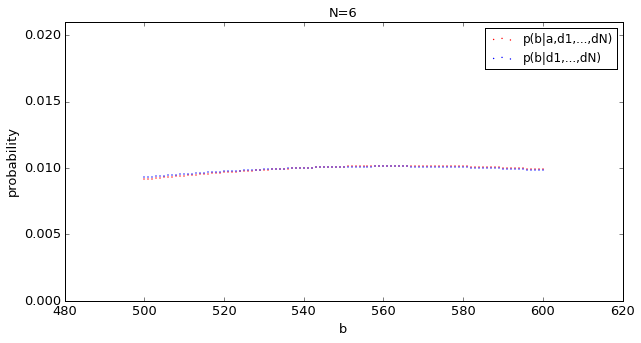
\includegraphics[width=8cm, height=4cm]{graphs/m3_ex_n6.png} &
                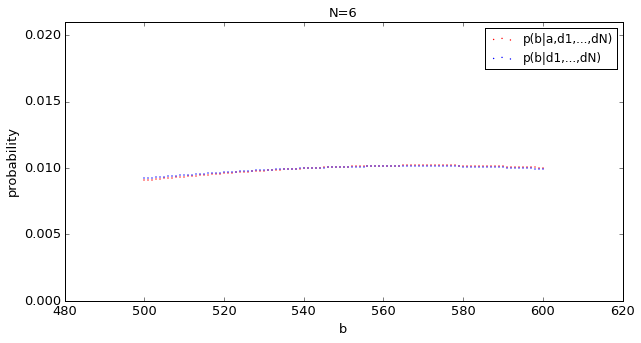
\includegraphics[width=8cm, height=4cm]{graphs/m4_ex_n6.png} \\
                
                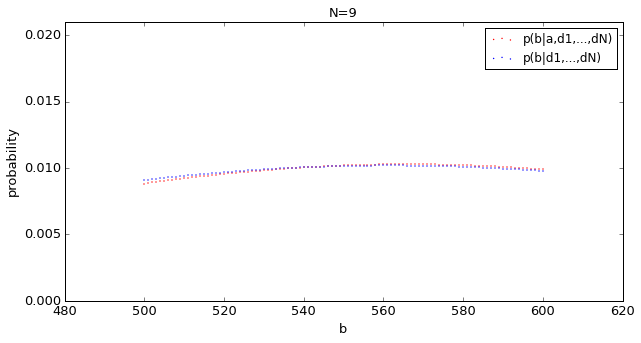
\includegraphics[width=8cm, height=4cm]{graphs/m3_ex_n9.png} &
                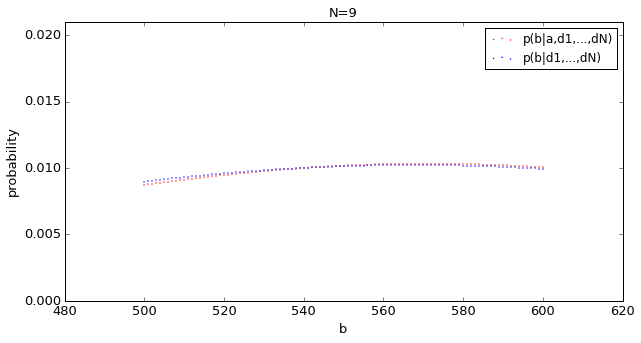
\includegraphics[width=8cm, height=4cm]{graphs/m4_ex_n9.png} \\
                
                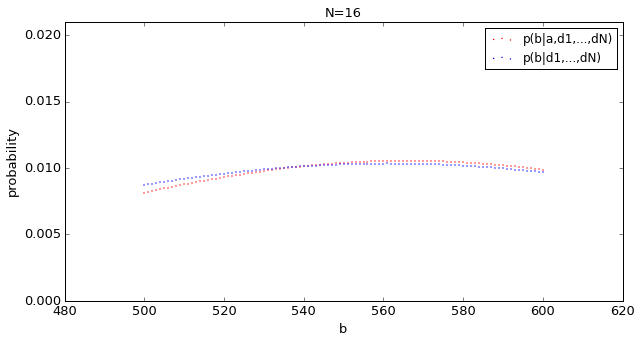
\includegraphics[width=8cm, height=4cm]{graphs/m3_ex_n16.png} &
                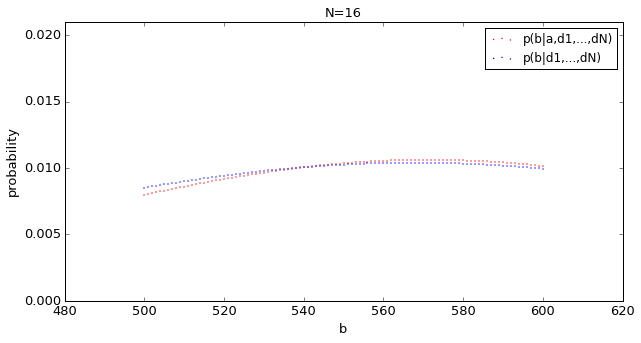
\includegraphics[width=8cm, height=4cm]{graphs/m4_ex_n16.png} \\
                
                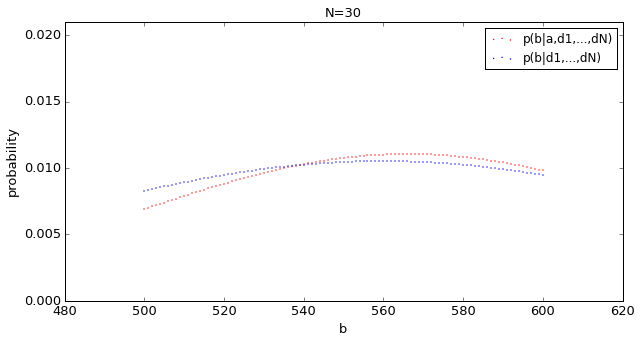
\includegraphics[width=8cm, height=4cm]{graphs/m3_ex_n30.png} &
                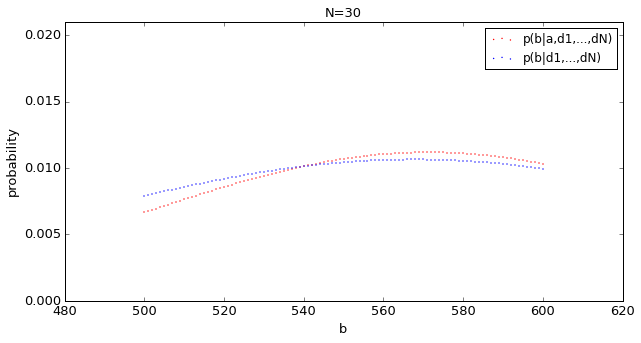
\includegraphics[width=8cm, height=4cm]{graphs/m4_ex_n30.png} \\
                
                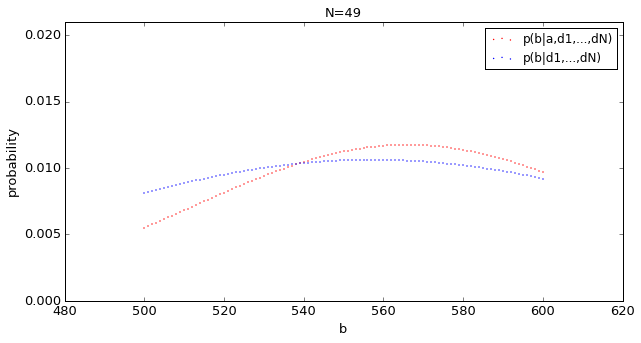
\includegraphics[width=8cm, height=4cm]{graphs/m3_ex_n49.png} &
                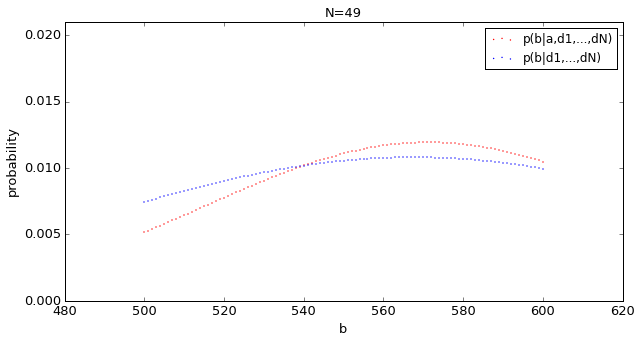
\includegraphics[width=8cm, height=4cm]{graphs/m4_ex_n49.png} \\
			\end{tabular}
			\end{center}
			
			Далее, если все $d_i$ равны матожиданию своего априорного распределения, то погрешность между моделю 3 и моделю 4 пренебрежимо мала. Это можно объяснить тем, что берутся средние значения отметившихся студентов, тем самым оценка $b$ выше около матожидания $b$. И так как сумма биномиальных распределений и распределение Пуассона имеют одинаковые матожидания, то модели являются практический одинаковыми. Также известное значение $a$ практический не меняет распределение.
			
		
		\newpage
		\subsection{Замер времени работы}
		\begin{center}
		\begin{tabular}{| l | c | c |}
			\hline
			& Модель 3 & Модель 4 \\
			\hline
			$p(c_n)$ & 124 ms & 35.4 ms \\
			\hline
			$p(d_n)$ & 140 ms & 55.9 ms \\
			\hline
			$p(b|d_1, ..., d_N)$ & 35.1 s & 36.1 s \\
			\hline
			$p(b|a, d_1, ..., d_N)$ & 2.17 s & 2.25 s \\
			\hline
		\end{tabular}
		\end{center}
	
		Времена работы при нахождении $p(c_n)$ и $p(d_n)$ различаются в 2-3 раза, так как в модели 3 нужно делать свертку, что является трудоемкой задачей. А при подсчете  $p(b|d_1, ..., d_N)$ и $p(b|a, d_1, ..., d_N)$ времена работы практический одинаковые, но большие. Поэтому разница времени для моделей из-за свертки не влияет на общее время.
		

	\newpage
	\section{Заключение}
		В итоге встает вопрос о выборе модели. Времена подсчета $p(b|d_1, ..., d_N)$ и $p(b|a, d_1, ..., d_N)$ для двух моделей одинаковые. Поэтому смотрим на погрешность приближения моделей. В случае, если $d_1 = ... = d_N = \mathbb{E} d_N$, то особой разницы в моделях нет. А в общем случае когда выборка $d_1, ..., d_N$ генерится случайным образом, то модель 4 дает большие погрешности, что является причиной не использовать эту модель. В итоге, т.к. время работы моделей одинаковые, лучше использовать модель 3.
		
		P.S. Если бы код писался более оптимально, то модель 4 была бы быстрее, т.к. не надо было бы считать свертку. Но при этом эта модель давала бы большие погрешности.
		

\end{document}
